\documentclass{article}
% \documentclass[review]{elsarticle}
\usepackage{epsfig}
\usepackage{amsmath}
\usepackage{mathtools}
\usepackage{algorithm}
\usepackage[algo2e,noend]{algorithm2e}
\usepackage[compatible,noend]{algpseudocode}
\usepackage{enumitem}
\usepackage{xspace}
\usepackage[table,xcdraw]{xcolor}
\usepackage{amsfonts}
\usepackage{pifont}
\usepackage{bbding}
\usepackage[english]{babel}
\usepackage{adjustbox}
\usepackage{tikz}
\usetikzlibrary{automata, topaths, calc, positioning, shapes, backgrounds, fit, matrix}
\usepackage{caption}
\usepackage{tabularx}
\usepackage[T1]{fontenc}
\usepackage{natbib}
\usepackage{datatool}
\usepackage{array}
\usepackage{pgfplotstable}
\pgfplotsset{width=7cm,compat=newest}
\usepackage{booktabs}
\usepackage{longtable}
\usepackage{pdflscape}
\usepackage{afterpage}
\usepackage{capt-of}
\usepackage{multirow}
\usepackage{float}
\usepackage[text={15cm,21cm},centering]{geometry}
\usepackage{setspace}
\usepackage{array}
\allowdisplaybreaks
\usepackage{lineno}
\usepackage{tkz-graph}
\usepackage{breqn}
\tikzset{
base/.style = {shape=rectangle, 
                      anchor=center,minimum size=5mm, 
                     align=center,
                     top color=white, ,inner sep=0ex,
                     minimum size=5mm
                     },
    LC11/.style =   {  base,   
                    text width=3em, 
                    bottom color=brown!100,
                    },
    UC11/.style = {     base,    
                    text width=5em, 
                    bottom color=brown!100,
                    align = right,
                },
    LC12/.style =   {  base,   
                    text width=1em, 
                    bottom color=orange!100,
                    },
    UC12/.style = {     base,    
                    text width=2.5em, 
                    bottom color=orange!100,
                },
    LC21/.style =   {  base,   
                    text width=1.5em, 
                    bottom color=brown!100,
                    },
    UC21/.style = {     base,    
                    text width=3.5em, 
                    bottom color=brown!100,
                },
    LC22/.style =   {  base,   
                    text width=4em, 
                    bottom color=blue!100,
                    },
    UC22/.style = {     base,    
                    text width=7em, 
                    bottom color=blue!100,
                    align = left,
                },
    UC221/.style = {     base,    
                    text width=3.5em, 
                    bottom color=blue!100,
                    % color=blue!100,
                    outer xsep=0em,
                    % align = right,
                },
                UC231/.style =   {  base,   
                    text width=1.5em, 
                    bottom color=blue!100,
                    },
    LC23/.style =   {  base,   
                    text width=1.5em, 
                    bottom color=orange!100,
                    },
    UC23/.style = {     base,    
                    text width=2.em, 
                    bottom color=orange!100,
                },
  env/.style      = {base, font=\ttfamily\normalsize},
label/.style   = {base,font=\ttfamily\normalsize, text width = 8em, 
  inner sep=0em, rounded corners=1mm,bottom color=gray!80,},
  dummy/.style    = {circle,draw}
}


\newtheorem{theorem}{Theorem}[section]
\newtheorem{lemma}[theorem]{Lemma}
\newtheorem{proposition}[theorem]{Proposition}
\newtheorem{corollary}[theorem]{Corollary}
\newtheorem{definition}[theorem]{Definition}
\newcommand{\pcmaxc}{P$|\mbox{\em cont}|$C$_{\max}$\xspace}
\newcommand{\alns}{adaptive large neighborhood search\xspace}
\newcommand{\Alns}{Adaptive large neighborhood search\xspace}
\newcommand{\F}{$\mathcal{F}$\xspace}
\newcommand{\B}{$\mathcal{B}$\xspace}
\newcommand{\C}{$\mathcal{C}$\xspace}
\newcommand{\Lb}{$\mathcal{L}$\xspace}
\newcommand{\D}{$\mathcal{D}$\xspace}

\renewcommand{\algorithmicforall}{\textbf{for each}}
\SetKwFor{ForEach}{for each}{}{}%
\renewcommand{\algorithmiccomment}[2][1\linewidth]{%
\leavevmode\hfill\makebox[#1][l]{/* \textbf{~#2} */}}
\renewcommand{\algorithmicrequire}{\textbf{Input:}}

\renewcommand{\tabcolsep}{4pt}

\modulolinenumbers[1]
\linenumbers

\oddsidemargin=0.5in
\topmargin=-0.25in
\textwidth=5.5in
\textheight=8.25in

%\journal{European Journal of Operational Research}

%\begin{frontmatter}

		
\title{A GRASP algorithm for the concrete delivery problem. }
\author{Ousmane Ali$^{(1)}$, Jean-Fran\c cois C\^ot\'e$^{(2)}$, Leandro C.~Coelho$^{(3)}$\\
 $(1)$ {\tt nassoma-wattara-ousmane.ali.1@ulaval.ca}\\
 $(2)$ {\tt Jean-Francois.Cote@fsa.ulaval.ca}\\
 $(3)$ {\tt Leandro.Coelho@fsa.ulaval.ca}\\
}

% \date{\today}

\begin{document}
\maketitle
\begin{abstract}
    %We study the daily scheduling of concrete delivery. Truck drivers are dispatched based on assignment priority and remaining working time over the horizon planning. A customer may be served from several available production plants. Due to the heterogeneity of the fleet, the number of visits to a customer location is not known ahead of time. The objective is to schedule drivers while minimizing travel times, waiting duration, idle time, and overtime. We solve this problem using a greedy randomized adaptive search procedure. Computational experiments with real data show the performance of our methods over the approach used by a local company. 
\end{abstract}

% \begin{keyword}
\noindent{\textbf{Keywords:} Vehicle routing; scheduling; ready-mixed concrete; concrete delivery
% \end{keyword}

%\end{frontmatter}

\section{Introduction}
\label{sec:intro}

Construction projects involve a huge movement of equipment, people, and materials. Among the latter, concrete is one of the most used. It is a perishable product with many factors affecting its quality \citep{sinha_quality_2021}. It comes in two types: ready-mixed concrete (RMC) and site-mixed concrete (SMC). As its name implies, SMC is produced on the spot using raw materials (water, aggregates, and cement) stored on the construction site, while RMC is manufactured in a batch plant and delivered to the construction site. SMC can avoid delays caused by road traffic, but has a slower and more difficult production process, requires storage for mixing materials and equipment, and is suitable for low amounts of concrete. It is quite the opposite for the RMC, which has better quality and benefits from lower production cost \citep{muresan_comparing}. Nevertheless, the batch plant manager must employ a fleet of high-cost revolving drum trucks (concrete mixers) to dispatch the ready-mixed concrete. Hence, the key to reaping the RMC benefits is to ensure efficient and prompt delivery on the construction site.

Concrete delivery under the form of RMC is subject to many operational constraints that make it a challenging problem met in Operations Research and addressed by the Concrete Delivery Problem (CDP). In this paper, we study a variant of the Concrete Delivery Problem to schedule the daily production and dispatching of RMC for a company located in the province of Quebec, Canada. This company produces RMC in multiple batching plants with different production rates, using a fleet of concrete mixers of various capacities. Each plant has its specific fleet, but a truck can load elsewhere if deemed necessary, except it must return to its home plant at the end of the day. They own two types of trucks with different capacities but can call on an external fleet when needed. They serve a construction site from any batch plant, with the first delivery starting at the time specified by the customer.  Loading and unloading a concrete mixer depends on the truck capacity, a plant's loading, and a construction site's unloading rate, respectively. The problem is like the one addressed in \cite {schmid2009hybrid, schmid2010hybridization}, except for the plant's production rate and the lack of unloading instrumentation in our case. Also, as per union rules, they assign a truck driver to a delivery task based on his seniority. The company uses a centralized dispatcher system to schedule all daily orders, but this system has issues satisfying all daily demands without using an external fleet.

According to \cite{blazewicz2019handbook}, the concrete delivery problem combines vehicle routing with scheduling issues to plan routes to deliver concrete from batch plants (depots) to customers' construction sites. Ready-mixed concrete is an on-demand product with a short life cycle from production through end use. It cannot be stored and cannot stay too long in a truck, or it will harden. Hence, concrete mixers must deliver RMC at the planned construction site shortly after its production. RMC production and delivery is then an example of a Just-In-Time (JIT) production system in construction \citep{tommelein1999just}. A customer quantity requirement is often greater than the truck size and must be fulfilled by multiple deliveries. In that sense, CDP is like the Vehicle Routing Problem (VRP) with split delivery (VRPSD) \citep{archetti2008split}, except that the same truck may visit a customer more than once.

Since concrete hardens quickly, in case of multiple deliveries, back-to-back deliveries must be continuous or at least close in time to avoid the problem of cold joint that negatively affects the quality of the concrete. Customers request to be served within a specific time window, complicating truck loading schedules when a plant can only load one truck at a time. Likewise, often only one truck can unload at a time at a customer location, sometimes leading to concrete mixers queuing and waiting their turn to deliver. Furthermore, with trucks of varied sizes, loading, travel, and unloading times that may be uncertain, the Concrete Delivery Problem is a complex problem to solve and has been proven by \cite{asbach2009analysis} to be NP-hard. With a single batching plant, the objective is to maximize the service level (serve all customers and avoid delays between subsequent deliveries and truck queuing). With additional production centers to choose from, a minimization of the total travel time is added to the objective. %However, these objectives can be conflictive.   
% We go a step further to add human constraints to the CDP, overtime, minimum and maximum hour of work, 

The remainder of the paper is organized as follows. Section \ref{lit_review} presents an overview of the CDP-related literature.  Section \ref{desc_form} provides a formal description of the problem. Then in Section \ref{method}, we describe the Greedy Randomized Search Procedure (GRASP) algorithm and the constructive heuristics we design to solve this variant of the CDP. Computational experiments and our conclusions follow in Sections \ref{comp_exp} and \ref{concl}, respectively.


\section{Literature review}
\label{lit_review}

A text mining approach for reviewing the ready-mixed concrete literature \citep{maghrebi2015text} showed that concrete technology and material science are the main core of research in this area. The first academic research on concrete batching and delivery began in the late 1990s. \cite{tommelein1999just} describe RMC as a prototypical example of a Just-In-Time production system in construction and identify two practices occurring when delivering it. An alternative is for the customer to haul the product from the batch plant with their concrete mixer. The other approach is where the batch plant delivers the concrete to the customer's location. This latter approach is the one studied in all related papers found in the literature.

Several works on the CDP mainly focussed on Simulation related methods, either standalone \citep{zayed2001simulation, wang2001scheduling, tian_simulation_based_2010, panas_simulation_based_2013, galic2016simulation}, etc. or hybridized with optimization methods \citep{feng2004optimizing, lu2005optimized, feng_integrating_2006}, etc. to schedule and dispatch concrete production and delivery. \cite{wang2001scheduling} developed a simulation model to reveal the effect and value of the concrete mixers' inter-arrival time on the productivity of hired unloading equipment on site. With a combination of Genetic Algorithm (GA) and simulation process, \cite{feng2004optimizing} tried to minimize the total waiting time for trucks at a customer site. Loading trucks with identical capacities is carried out at the same batch plant. Loading and unloading durations are fixed. GA is used to find the most efficient and effective loading sequence of RMC trucks to be assigned to different construction sites. The simulation process determines the loading, arrival, departure, and waiting time of trucks and thus evaluates the cost of each dispatching sequence. They evaluated the method using data from a batch plant in Taiwan with up to nine customers served. \cite{mayteekrieangkrai2015optimized} solved the same problem with the same data using a bee algorithm (BA) and found better solutions than the GA. \cite{lu2005optimized} used the same combination of GA and simulation to decide on the optimal number of concrete mixers to be deployed together with an optimal schedule for batching and delivering concrete. Their objective is to minimize the site crew idle times due to late concrete deliveries plus truck queuing time. The particularity of this setting is that mortar useful for unloading pump lubrication must be delivered on-site before concrete. Therefore, mortar batching and delivery are also modeled in the simulation. Finding the best RMC truck size was also the purpose of the discrete-event simulation model proposed by \cite{panas_simulation_based_2013}.

Besides simulation-based methods, we find in the literature works using metaheuristics \citep{faria2006distributed, misir2011selection, maghrebi2016sequential, yang2022concrete}, exact methods \citep{yan2007optimal, kinable2014concrete}, matheuristics \citep{schmid2009hybrid, schmid2010hybridization}, Benders Decomposition \citep{maghrebi2014benders}, Column Generation (CG) \citep{maghrebi2014solving, maghrebi2016column}, Lagrangian relaxation \citep{narayanan2015using}, and machine learning approach \citep{graham2006modeling, maghrebi2014exploring, maghrebi2016matching}.
\cite{matsatsinis2004towards} designed a decision support system (DSS) for the dynamic routing of both concrete and pumps that may be necessary for some sites to help the concrete unloading. Three plants are available, but vehicles fulfilling the same order must all load at the same plant. An order that cannot be executed may be postponed for the next day. The routing of the pumps is modeled as a multi-depot VRP with time windows. \cite{naso2007genetic} proposed a sequential GA method combined with constructive heuristics to solve a more general variant of the CDP. In this problem, besides batching concrete delivered to a customer site, the plant's production schedule must include orders picked up by the customers themselves. The algorithm first schedules the plant loading operations before scheduling truck job deliveries. A non-linear model minimizing transportation costs, waiting times, outsourced costs, and overtime work is also developed. The authors ran experiments using real-world instances of a concrete supply chain in the Netherlands. They found a reduction in the number of requests redirected to external companies. \cite{yan2007optimal} also emphasized overtime considerations in their paper scheduling RMC for one batching plant with two loading docks. Overtime wages are paid for factory and construction site operations after 4 PM. A mixed integer programming (MIP) model on a time-space network is developed to minimize travel times and operating costs at both normal and overtime working hours at the plant and the construction sites. Real data consisting of 3 days of operation is tested using a two-stage algorithm. First, they solved the MIP relaxation with CPLEX. Then they simplify the original model by fixing some decision variables before solving it. This algorithm seems to improve the actual plant operation by 10\%.
A time-space network is the principal component of the real-time DSS developed by \cite{durbin2008or} to solve a dynamic CDP every five minutes. The DSS can receive new orders, schedule them on the fly, and deal with unexpected events such as plant closures, truck breakdowns, delays in transportation times, etc. Combined with a Tabu Search (TS) heuristic to warm start CPLEX, the model is performant enough to solve instances with up to 1,500 loads per day with up to 250 trucks. The authors consider the case of a customer who places two orders, with the first being completed before the second starts. The real-time planning and monitoring of CDP are studied more in detail by \cite{garza2021dynamic} in his thesis. Another variant of the CDP is modeled by \cite{schmid2009hybrid} as an integer multicommodity network flow (MCNF) problem on a time-space network. In this paper, concrete is delivered using a heterogeneous fleet of vehicles, and each plant can load an illimited number of trucks simultaneously. Among the trucks, some have specialized equipment and must arrive first at certain construction sites to assist concrete-mixers unloading. The objective is to fulfill all orders, minimize the travel cost, and avoid delays between two consecutive unloading operations for an order. The model is typically solved using a matheuristic algorithm that combines the MCNF with a variable neighborhood search (VNS) heuristic. The method can solve large problem instances with more than 60 orders per day quickly without encountering any memory issues. The same problem is addressed by \cite{schmid2010hybridization}. The authors proposed a MIP model combined with a VNS and a very large neighborhood search (VLNS) to develop two matheuristics approaches. Comparisons between both matheuristics and a standalone VNS show that the former methods are much better and suitable for solving larger problem instances. These methods also provide better solutions for small to medium instances than the matheuristic used in \cite{schmid2009hybrid}. A pure VNS approach with the same problem but without the use of instrumentation has been applied by \cite{payr2009optimizing}.

Regarding objectives, most authors have been interested in minimizing travel time and delays between consecutive deliveries. Some authors, however, were more interested in maximizing only customer satisfaction. We find these situations in the works of \cite{durbin2008or, kinable2014concrete, kinable2014logic, sulaman2017simulated}.
\cite{kinable2014concrete} introduce a general MIP and constraint programming (CP) models of the CDP reflecting the main constraints commonly found in all CDP works: time lag and no overlapping between consecutive deliveries, covering of all customers' demands, delivery time window, and heterogeneous fleet. However, the model did not include constraints limiting the time that concrete may reside in a truck. The authors also propose a constructive heuristic that schedules the visits to the customers one by one according to the start time of the visit and the truck capacity. The procedure is invoked multiple times for different permutations of the customer's order which is determined using the steepest descent (SD) local search procedure. One of the paper's main contributions is the creation of the first public test instances for the CDP with up to 50 customers, four batching plants, and 20 concrete mixers. They found the CP model to be highly effective in finding high-quality solutions in relatively little time or improving existing schedules, while the MIP model can be used to compute bounds, as it seems ineffective in solving large problem instances. Finally, the heuristic often yields good solutions in less than a second. A detailed analysis of the MIP model presented in cite{kinable2014concrete}and of two more compact models can be found in the thesis of \cite{hernandez_lopez_study_2020}. In \cite{kinable2014logic}, we find an attempt to solve the previous problem with a Logic Based Benders' approach. \cite{sulaman2017simulated} expand upon the SD heuristic proposed in \cite{kinable2014concrete}, proposing a Simulated Annealing (SA) with a Time-Slot Heuristic (TH). TH mechanism is to look for a slot between existing visits of a truck to schedule a new delivery instead of assigning it to the time slot strictly after the truck's latest assigned delivery. The goal is to reduce the large time gaps that can be present in a schedule created with SD due to ignoring the intermediate available time slots. Experimental results indicated that SATH outperforms SD in speed and solution quality. A generalization of the MIP model of \cite{kinable2014concrete} is addressed in \cite{asbach2009analysis}. This model simultaneously minimizes the total sum of travel costs and the penalty costs for customers with unfulfilled demand. A customer can request that all concrete deliveries come from the same plant or a subset of plants and that a delivery truck belongs to a subset of the vehicle fleet. The MIP model is used in a local search scheme as a black-box solver to reoptimize an incumbent solution in which a neighborhood operator has unfixed some variables.

%\cite{tzanetos2023systematic} present a systematic search and mapping review of the concrete delivery problem. this paper fills that gap by (a) performing a comprehensive search on the CDP, and (b) mapping out and categorizing the existing literature. Specifically, this paper provides an overview of the various methods of the literature, categorizing the problem formulations based on the literature’s different concepts,



\section{Problem description}
\label{desc_form}
The problem studied within this paper is about the distribution of ready-mixed concrete from a Canadian company operating in the greater Montreal area. Concrete order from a customer arrives at a central center and is assigned to one of the batching plants from where the product will be produced and delivered to the customer. We define an instance of our problem on a set of batching plants, a set of customer orders, and a set of drivers.

% \subsection*{Batching plants}

The company owns and operates a total of eight concrete batching plants located in different geographical areas. The loading bays in each plant can only accommodate one truck at a time, resulting in trucks lining up. Let $\mathcal{B}$ be the set of batching plants. The plants are heterogeneous, as each plant $b$ has its hourly loading rate $\tau^l_b$ which influences the loading time duration. After loading, a driver takes $\alpha_b$ minutes to adjust the concrete in his truck before departing to the customer site. Any batch plant can serve a construction site if the traveled time between them is less than the concrete lifespan $\delta$. Each plant has its assigned fleet, but it can get a vehicle from another plant or even hire an external fleet. If $q_i$ is the quantity of RMC loaded to customer $i$ from plant $b$, we compute the loading time duration $LD^b_i$ as

\begin{equation}
    \label{eq:LD}
    {LD}^b_i = \frac{q_i}{\tau^l_b}.
\end{equation}

% \subsection*{Customer orders}

A customer $i$ requests one or several types of concrete to be delivered to his construction site on a particular day for a total amount of $q_i$. When placing an order, he specifies the number of types of RMC $P_i \geq 1$, the quantity $q^p_i$ of concrete of each type $p$, the arrival time $a_i$ of the first concrete mixer, and the unloading rate $\tau^u_i$ at his site. $\mathcal{C}$ is the set of construction sites (customers) with a planned delivery for the day.

We refer to order $o^p_i$ as the request of customer $i$ to receive a type $p$ of concrete. If the amount of concrete exceeds any truck capacity, several deliveries are scheduled to satisfy an order. $n^p_i \geq 1$ is the number of deliveries needed to satisfy $o^p_i$. Let $d^p_{ij}$ be the $j_{th}$ visit with load $q^p_{ij}$ for order $o^p_i$. We represent the delivery of order $o^p_i$ by the visits to the ordered set of nodes $\mathcal{D}^p_i= (d^p_{i0},d^p_{i1},\cdots, d^p_{in^p_i})$. All quantities of a type of concrete must be thoroughly delivered before moving on to another type. The orders $o^p_i$ $(1 \leq p \leq P_i$) of a customer $i$ are not ordered. An order can start at any time, provided it is completed before delivering another. We represent the delivery of customer $i$ by the set $\mathcal{D}_i= (\mathcal{D}^{p^0}_i, \mathcal{D}^{p^1}_i,\cdots,\mathcal{D}^{p^{P_i}})$, where $p^l$ is the $lth$ order delivered. We define for the first node of $\mathcal{D}^{p^0}_i$ the time window $ \left\lbrack a_i, b_i  \right\rbrack$ to ensure that the first delivery of $i$ must be due at $a_i$. Once a plant is chosen to produce a customer's first order, it must be the provider of all subsequent orders of this customer.

To prevent cold joint in concrete, subsequent deliveries must be in just in time, or at least close in time. We define a maximum time lag $\gamma_i$ beyond which no next unloading operation should be allowed. The construction site unloading rate and the quantity to unload give the time necessary to discharge a truckload. The unloading time duration of $q^p_{ij}$ is
\begin{equation}
    \label{eq:UD}
    {UD}_{d^p_{ij}} = \frac{q^p_{ij}}{\tau^u_i}
\end{equation}

% \subsection*{Drivers}

%A driver is an important entity here, as we must incorporate some union constraints into our model. 
The company has two types of trucks with capacities of 8 and 12 $m^3$. A driver $k$ is assigned to a plant from where he starts and ends his shift day, and drives one concrete mixer of capacity $Q_k$. The set of drivers is $K=\cup_{b \in \mathcal{B}}K_b $, $K_b$ being the set of drivers scheduled to start their shift at the batching plant $b$. 

A driver must work between four and eight hours in normal time, plus optional overtime of two hours at most, during a scheduled day. A driver mainly loads RMC at his home plant but can still drive at other plants and load there if needed. Batching plant produces concrete on-demand with recipes specific to customers, which means that truck cannot hold orders for more than one client, even if it has spare capacity. Thus, a driver must refill at a plant between two consecutive deliveries. After unloading the RMC, a driver takes $\beta_k$ minutes to clean the concrete mixer before traveling to his next loading plant. When assigning a driver to a delivery, priority is given to the employees with the highest seniority.

For an order $o^p_i$, the number of deliveries $|D^p_i|$ is not known a priori, as we use a fleet with various capacities. However, we can compute the lower and upper bounds of $|D^p_i|$ using the capacities of the highest ($Q_{max}$) and smallest ($Q_{min}$) available trucks. The lower (upper) bound $\left\lceil \frac{q^p_i}{Q_{max}} \right\rceil$ $\left(\left\lceil \frac{q^p_i}{Q_{min}} \right\rceil \right)$ is the number of deliveries needed if we only use trucks of capacity $Q_{max}$ ($Q_{min}$).

% \subsection*{Model}

A solution to our problem is a set of decisions about truck loading schedules, driver assignments for different deliveries, and truck arrival times at construction sites for unloading. For a batching plant, the decision is to determine which driver should be loaded, when, and for which construction site. For a driver, the decision is the sequence of loading depots and delivering sites. And for a construction site, the arrival time of all daily scheduled deliveries. 

Let the binary variable $x^{bk}_{j}$ be $1$ if a driver $k$ loads at plant $b$ to serve the delivery node $j$. % $y_i=1$ if $i$ is completely served.
Let $SLT^{bk}_{j}$ and $ELT^{bk}_{j}$ be the start and end loading time of driver $k$ at plant $b$. $SUT_{j}$, $EUT_{j}$ be the start and end unloading time. $LTS^{bk}_{j}=\left[ SLT^{bk}_{j}, ELT^{bk}_{j} \right] $, and $UTS^{bk}_{j}=\left[ SUT^{bk}_{j}, EUT^{bk}_{j} \right]$ stand for the loading  and unloading operations timeslots. $AT_{j}$ is the arrival time of a driver at the node location.

\begin{alignat}{2}
    \label{eq:ELT}  ELT^{bk}_{j} &= SLT^{bk}_{j}+ LD^b_{j}\\
    \label{eq:S}         EUT_{j} & = SUT_{j} + UD_{j}
\end{alignat}

For each delivery node $j$, we define an expected delivery time $EDT_{j}$ of unloading operation, the driver waiting duration $W^k_{j}$, and the node waiting time $W_{j}$.


\begin{alignat}{3}
    \label{eq:ES} EDT_{d^{p^l}_{ij}} &=
          \begin{cases}
            a_i & \text{if $j=0$, $l=0$}\\
            E_{d^{p^l}_{ij-1}} & \text{ $j \geq 1$}\\
            E_{d^{p^{l-1}}_{in^{p^{l-1}}_i}}  & 
          \end{cases} &  \\
    \label{eq:Wd} W^k_{d^p_{ij}} &= \max\{0, SUT_{d^p_{ij}} - AT_{d^p_{ij}}\} & \\
    \label{eq:Wc} W_{d^p_{ij}} & = \max\{0, AT_{d^p_{ij}} - EDT_{d^p_{ij}}- \lambda_i \} &
\end{alignat}

% Parler de la reduction des W

We keep track of the working time of each driver $k$ with the variable $WT_k$. Parameters $N_t$ and $O_t$ are the normal and overtime working hours. $M_t$ is the minimum working time for a day. $\Gamma_1$ and $\Gamma_2$ are the incurred penalties when a driver works less than $M_t$ and more than $N_t$.
\begin{equation}
    \forall k \in K, WT_k \leq O_t 
\end{equation}

The objective is to minimize the traveled distance,
 of delivered concrete to the satisfied customers as in

\begin{equation}
    \min \smashoperator{\sum_{i,j}}{t_{ij}x_{ij}}
\end{equation}


The cost to travel between two nodes ($i$, $j$) is the travel time $t_{ij}$. COST...



\paragraph*{}
Let us consider the small instance illustrated in Figures~\ref{fig_Example} and \ref{fig:ganttExample}. Two batching plants $B_1$ and $B_2$ with three drivers serve two construction sites. Customer $C_1$ requests one order of $q^1_1=12$ m$^3$. Customer $C_2$ requests three orders of $q^1_2=3$, $q^2_2=11$, and $q^3_2=1$ m$^3$ of three different types of concrete. $B_1$ has two drivers ($D_1$, $D_2$) using concrete mixers of capacity 8 m$^3$, and $B_2$ has $D_3$ of capacity 12 m$^3$. Figure~\ref{fig_Example} depicts the concrete mixers flow in the network. We schedule $D_1$ and $D_2$ to respectively deliver 8 and 4 m$^3$ to $C_1$. We select $o^2_2$ as the first order of $C_2$ to deliver. $D_3$ travels to $B_1$ to load $q^2_2$, then visits $C_2$ before returning to his home plant. Meanwhile, after their first trip,  $D_1$ and $D_2$ deliver the remaining orders of $C_2$.

Figure~\ref{fig:ganttExample} shows the sequence of loading and unloading operations. The first deliveries of $C_1$ and $C_2$ are timely and there is no gap between the two deliveries received by $C_1$. There is a delay between the end of the first delivery and the start of the second delivery of $C_2$, however, it is less than the maximal time lag of 20 minutes defined for this example.


\begin{figure}[!ht]
    % \caption{Solution of an instance with two plants, two construction sites, four orders, and three drivers.}
    \vspace*{-10mm}

    \centering
    \begin{adjustbox}{max width=0.85\textwidth}
      
  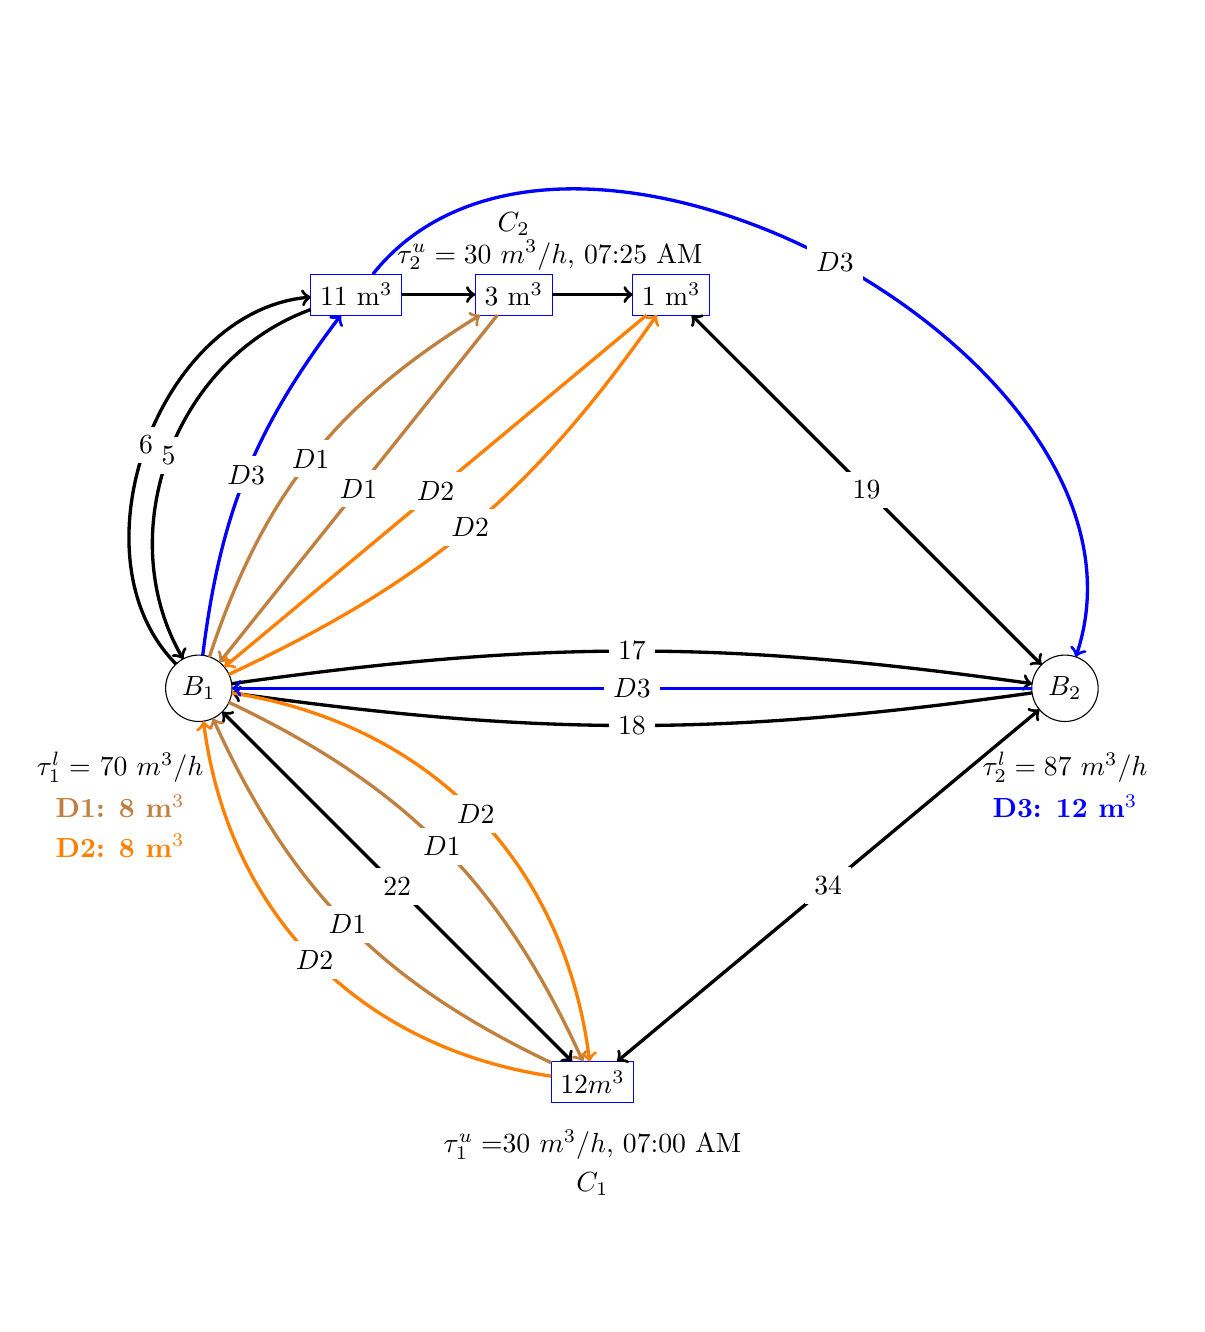
\begin{tikzpicture}
    \SetUpEdge[lw = 1.2pt,
        labelcolor = white,
        % labelstyle = {draw}
    ]
    \tikzstyle{LabelStyle}=[fill=white]

    \SetGraphUnit{5}
    \GraphInit[vstyle=Normal]
    \tikzset{VertexStyle/.style = {shape = circle,text = black,minimum size = 24 pt,draw = black}}
    \Vertex[L={$B_1$}]{D1}
    \tikzset{VertexStyle/.style = {shape = circle,text = black,minimum size = 10 pt,draw = blue}}
    \tikzset{VertexStyle/.style = {shape = rectangle,text = black,minimum size = 10 pt,draw = blue}}
    \Vertex[x=2,y=5,L={11 m$^3$}]{C21}
    \EA[unit=2.0,L={3 m$^3$}](C21){C22}
    \EA[unit=2.0,L={1 m$^3$}](C22){C23}
    \tikzset{VertexStyle/.style = {shape = rectangle,text = black,minimum size = 10 pt,draw = blue}}
    \SOEA[L={$12m^3$}](D1){C1}
    \tikzset{VertexStyle/.style = {shape = circle,text = black,minimum size = 24 pt,draw = black}}
    \SOEA[L={$B_2$}](C23){D2}
    % %  \SetVertexArt
    \tikzset{VertexStyle/.style = {shape = circle,text = black,minimum size = 10 pt}}
    \SO[unit=0.8,L={$\tau^u_1=$30 $m^3/h$, 07:00 AM}](C1){tau1}
    \SO[unit=0.5,L={\textbf{$C_1$} }](tau1){o1}
    
    \NO[unit=0.9,L={\textbf{$C_2$}}](C22){C2}
    \SOEA[unit=0.4,L={\textcolor{white}{  } $\tau^u_2=30$ $m^3/h$, 07:25 AM}](C2){tau2}

    \tikzset{VertexStyle/.style = {shape = rectangle,text = black,minimum size = 10 pt}}
    \SOWE[unit=1.,L={$\tau^l_1=$ 70 $m^3/h$}](D1){cap1}
    \SO[unit=0.5,L={\textbf{\textcolor{brown}{D1: 8 m$^3$}}}](cap1){driver11}
    \SO[unit=0.5,L={\textbf{\textcolor{orange}{D2: 8 m$^3$}}}](driver11){driver12}
    \SO[unit=1,L={$\tau^l_2= 87$ $m^3/h$}](D2){cap2}
    \SO[unit=0.5,L={\textbf{\textcolor{blue}{D3: 12 m$^3$}}}](cap2){driver2}
    %%%%%%% Edge
    \tikzset{EdgeStyle/.style={->}}
    \Edge[](C21)(C22)
    \Edge[](C22)(C23)
    \tikzset{EdgeStyle/.style={<->,bend left=0}}
    \Edge[label=$22$](D1)(C1)
    \tikzset{EdgeStyle/.style={<->}}
    \Edge[label=$19$](D2)(C23)
    \Edge[label=$34$](D2)(C1)
    \tikzset{EdgeStyle/.style={->}}
    \tikzset{EdgeStyle/.append style = {bend left = 8}}
    \Edge[label=$17$](D1)(D2)
    \Edge[label=$18$](D2)(D1)
    \tikzset{EdgeStyle/.append style = {bend left = 65}}
    \Edge[label=$6$](D1)(C21)
    \tikzset{EdgeStyle/.append style = {bend right = 50}}
    \Edge[label=$5$](C21)(D1)
    \tikzset{EdgeStyle/.style = {->,bend left = 20,draw=brown}}
    \Edge[label=$D1$](D1)(C1)
    \Edge[label=$D1$](C1)(D1)
    \tikzset{EdgeStyle/.style = {->,bend left = 37,draw=orange}}
    \Edge[label=$D2$](C1)(D1)
    \Edge[label=$D2$](D1)(C1)

    \tikzset{EdgeStyle/.style = {->,bend left= 20,draw=brown}}
    \Edge[label=$D1$](D1)(C22)
    \tikzset{EdgeStyle/.style = {->,bend left= 0,draw=brown}}
    \Edge[label=$D1$](C22)(D1)
    
    \tikzset{EdgeStyle/.style = {->,bend left = 0,draw=orange}}
    \Edge[label=$D2$](C23)(D1)
    \tikzset{EdgeStyle/.style = {->,bend left = -15,draw=orange}}
    \Edge[label=$D2$](D1)(C23)
    

    \tikzset{EdgeStyle/.style = {->,,draw=blue}}
    \Edge[label=$D3$](D2)(D1)
    \tikzset{EdgeStyle/.style = {->,bend left = 15,draw=blue}}
    \Edge[label=$D3$](D1)(C21)
    \tikzset{EdgeStyle/.style = {->,bend left = 80,draw=blue}}
    \Edge[label=$D3$](C21)(D2)
    \end{tikzpicture}
    \end{adjustbox}
    \vspace*{-10mm}
    % }
    \caption{Solution of an instance with two plants, two construction sites, four orders, and three drivers.}
    \label{fig_Example}

\end{figure}

\begin{figure}[!htb]
    \centering
    
    \vspace*{-0mm}
    \begin{adjustbox}{max width=0.85\textwidth}
        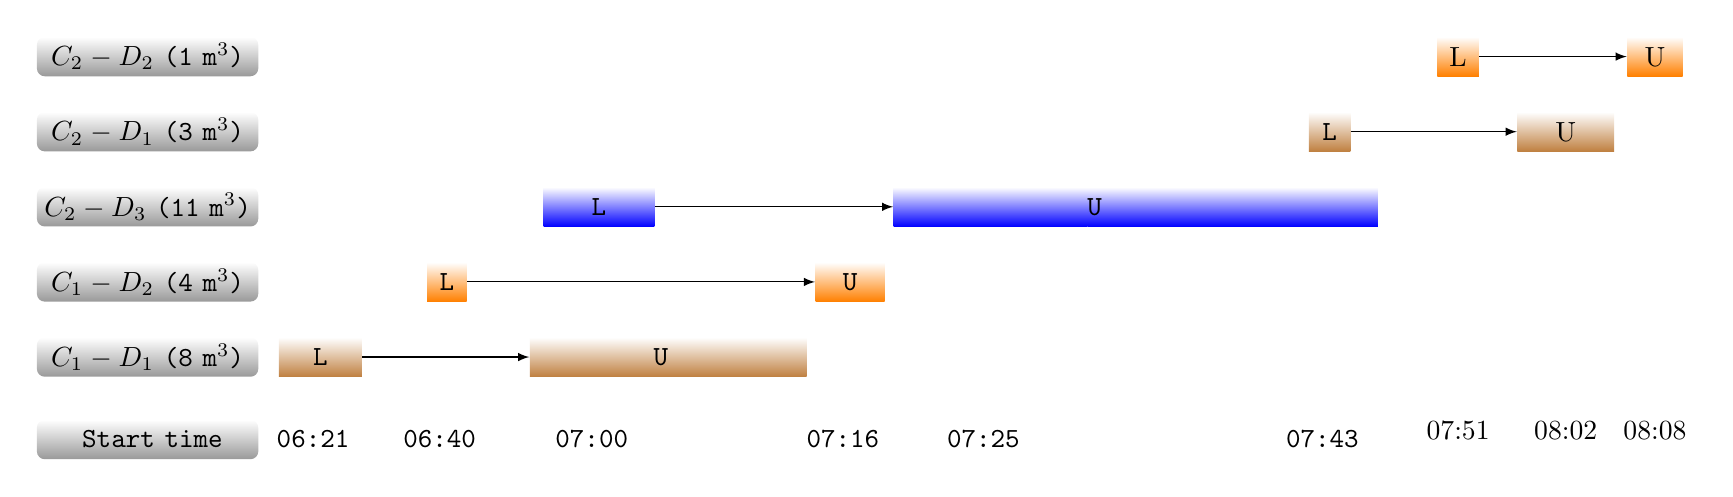
\begin{tikzpicture}[-latex]
            \matrix (chart)
            [
            matrix of nodes, nodes in empty cells,
            column sep      = 0em,
            row sep         = 3ex,
            column 1/.style = {nodes={label}},    column 2/.style = {},       column 3/.style = {nodes={env}},      column 4/.style = {nodes={env}},         column 5/.style = {nodes={env}},         column 6/.style = {nodes={env}},           column 7/.style = {nodes={env}},           column 8/.style = {nodes={env}},           column 9/.style = {nodes={env}},           column 10/.style = {nodes={env}},         column 11/.style = {nodes={env}},           column 12/.style = {nodes={env}},    column 13/.style = {nodes={env}}
            ]
            {
            $C_2-D_2$ (1 m$^3$) &
            &   &   &   &   &   &   &   &   &   &   &   &            |[LC23]| L &            &       &     |[UC23]| U \\
            $C_2-D_1$ (3 m$^3$) &           &      &        &        &           &            &            &
            &
            &
            &
            |[LC21]| L &
            &
            &
            &
            |[UC21]| U &
            \\
            $C_2-D_3$ (11 m$^3$) &
            &
            &
            &
            &
            &
            |[LC22]| L &
            &
            &
            |[UC22]| &
            |[UC22]|U  &
            |[UC221]|  &
            &
            &
            &
            &
            \\
            $C_1-D_2$ (4 m$^3$) &
            &
            &
            &
            |[LC12]| L &
            &
            &
            &
            |[UC12]| U &
            &
            &
            &
            &
            &
            &
            &
            \\
            $C_1-D_1$ (8 m$^3$) &
            &
            |[LC11]| L &
            &
            &
            &
            |[UC11]|U &
            |[UC11]| &
            &
            &
            &
            &
            &
            &
            &
            &
            \\
            \vspace*{-10em}
            Start time &&
            06:21 &
            &
            06:40 &
            &
            07:00 &
            &
            07:16 &  07:25 &
            &
            07:43 &
            &
            07:51 &
            &
            08:02 & 08:08 \\
            };
            % \node[fit={(chart-3-10) (chart-3-12)},style=UC22]{U};
            \draw (chart-5-3) edge (chart-5-7);
            % \draw (chart-5-8.3) edge (chart-2-12);
            \draw  (chart-4-5) edge (chart-4-9);
            % \draw  (chart-4-9) edge (chart-1-14);
            \draw  (chart-3-7) edge (chart-3-10);
            \draw  (chart-2-12) edge (chart-2-16);
            \draw  (chart-1-14) edge (chart-1-17);

        \end{tikzpicture}
    \end{adjustbox}
    \caption{Schedule of the instance of Figure~\ref{fig_Example}.}
    \label{fig:ganttExample}
\end{figure}


\section{Constructive heuristics and GRASP}
\label{method}

We now present the solution approach we implement to solve this variant of the Concrete Delivery Problem. Our method consists in constructing feasible solutions for the CDP with randomized heuristics and iteratively calling these heuristics in the greedy randomized adaptive search procedure (GRASP) metaheuristic.

In this section, we represent the scheduling of a delivery node $d^p_{ij}$ as a pair of loading $l_{d^p_{ij}}$ and unloading $u_{d^p_{ij}}$ tasks. We then refer to a solution $S$ as a set of loading and unloading tasks performed by a set of drivers during a particular day.
\begin{alignat*}{2}
    l_{d^p_{ij}} &= \left\lbrace (b,k,q^p_{ij},LTS^{bk}_{d^p_{ij}}), b \in \mathcal{B}, k \in K \right\rbrace \\
    u_{d^p_{ij}} & =  (k,A_{{d^p_{ij}}}, UTS_{{d^p_{ij}}}), k \in K  \} \\
    S &=\left\lbrace \cup _{1 \leq p \leq n^p_i} \cup _{1 \leq j \leq |D^p_i|} (l_{d^p_{ij}},u_{d^p_{ij}}), i \in \mathcal{C} \right\rbrace
\end{alignat*}
 

\subsection{GRASP algorithm  }

The GRASP algorithm is an iterative suite of constructive and local search algorithms introduced by \cite{feo1995greedy}. For each iteration, a feasible solution $S$ is built using a greedy randomized algorithm. Then a local search algorithm investigates the neighborhood of  $S$ to find a local optimum. The pseudo-code of Algorithm~\ref{alg_grasp} shows that the procedure returns the best overall solution (for a minimization problem) after some stopping conditions (time limit or a maximal number of iterations) are met. 

{\setstretch{1.0}
    {\small
        \begin{algorithm}[hpt]
            \caption{Pseudo-code of the GRASP algorithm }
            \label{alg_grasp}
            \DontPrintSemicolon
            \LinesNumbered
            \setcounter{AlgoLine}{0}
            \KwIn{ \textit{H}: List of constructive randomized heuristics }
            $S^* \leftarrow \emptyset$    \hspace{2mm}       $Cost(S^*) \leftarrow \infty$


            \While{Conditions not met}{
                $Cost(S') \leftarrow \infty$

                \ForEach { $h \in H$ }{

                    $S \leftarrow h(S)$

                    $S \leftarrow LocalSearch(S)$

                    \uIf{$Cost(S)< Cost(S')$}{
                        $S' \leftarrow S$

                        \uIf{$Cost(S')< Cost(S^*)$}{
                            $S^* \leftarrow S'$
                        }
                    }

                }
            }

            \KwRet{$S^{*}$}
        \end{algorithm}}
}
 

\subsection{Greedy randomized insertion algorithm}

As referred to in \cite{resende2019greedy}, the general outline of a greedy randomized algorithm used in the GRASP framework works as described in Algorithm~\ref{alg:greedyIns}. At each iteration, let's consider the set $CL$ of candidate delivery nodes that are not yet scheduled. We note that, for our problem, not all delivery nodes are candidates for insertion at each iteration, since deliveries of the same order are ordered, any order of a customer may be chosen, and it must be satisfied before switching to another order, and the number of visits to a customer is not known beforehand. We first initialize $CL$ with the first delivery of a random order for each customer. We create the set $CL'$ with elements of $CL$ we deem promising for a better solution. We evaluate the increase in the cost function when incorporating each $d \in CL'$ into the incumbent solution $s$ and create a restricted candidate list $RCL$ formed by nodes whose incremental costs are less than a defined threshold. From $RCL$, we randomly select the next delivery node to be incorporated into the incumbent solution and we determine its loading and unloading schedule with the procedure described in Algorithm~\ref{alg_ScheduleTask}. Next, we update $S$ and the remaining quantities of the order and customer. Then we add to $CL$ the next delivery node candidate. If an order $o^p$ is not yet fulfilled after the visiting $d^p_{ij}$, the candidate is the next delivery node $d^p_{ij+1}$. Otherwise, if the customer has remaining orders, the candidate is the first delivery node $d^{p'}_{i0}$ of another randomly selected order $p'$.

The greedy aspect of the GRASP is the creation of the $RCL$ set, the probabilistic aspect is the random selection in $RCL$, and the adaptive aspect is the update of $CL$ and the reevaluating of the incremental costs. We use the additional set $CL'$ because we noticed that restricting $CL$ to delivery nodes with the same demand, delivery due time, or overlapping unloading timeslots helps us intensify the search. Using $CL'$ also helps improve the algorithm complexity by reducing the number of nodes to evaluate. To diversify the search we simply remove the filter component. We thus obtain four greedy randomized insertion heuristics for our GRASP framework.

 {\setstretch{1}
%  {\small
     \begin{algorithm}[hbt]         
         \caption{Greedy randomized insertion algorithm }
         \label{alg:greedyIns}
         \DontPrintSemicolon
         \LinesNumbered
         \setcounter{AlgoLine}{0}
         \KwIn{  $S$: empty solution $S$}

         $CL \leftarrow \emptyset$

         \ForEach(customer i){}{
                Select a random order $o^p_i$

                $CL \leftarrow CL \cup \{d^p_{i0}\}$
        }

        
         \While{$CL \neq \emptyset$}{

            $CL' \leftarrow \text{Filter (CL)} $

            \ForEach( $d \in CL'$){}{
            
            $C(d) \leftarrow$ incremental cost of inserting $d$

            }
            $C_{min} \leftarrow min\left\lbrace C(d), \text{ } d \in CL' \right\rbrace $, $C_{max} \leftarrow max\left\lbrace C(d), \text{ } d \in CL' \right\rbrace $
            
            $RCL \leftarrow \left\lbrace d \in CL, \text{ } C(d) \leq C_{min} + \alpha (C_{max}-C_{min}) \right\rbrace $

            Select random delivery node $d^p_{ij}$ from $RCL$

            $l^p_{ij}$, $u^p_{ij}$ = ScheduleTasks($d^p_{ij},S$)

            $S \leftarrow S \cup (l^p_{ij}$, $u^p_{ij})  $

            $q_i \leftarrow q_i-q^p_{ij}$;  $q^p_i \leftarrow q^p_i-q^p_{ij}$

            \uIf {$q^p_i \neq 0$ }{

            $CL \leftarrow CL \cup \{d^p_{ij+1}\}$ 

            }
            \uElseIf{ $q_i \neq 0$}{

            Select another order $o^{p'}_i$

            $CL \leftarrow CL \cup \{d^{p'}_{i0}\} $

            }

            Update $CL$
         }
        \KwRet{$S$}
     \end{algorithm}
%  }
 }

 Algorithm~\ref{alg_ScheduleTask} takes as parameters a delivery node $d^p_{ij}$ and a partial solution and looks for a plant and a driver available for loading and unloading operations. For each driver $k$ and plant $b$ we simulate the loading and unloading operations while checking the concrete lifespan constraints, and the plant and driver availability. For each node, we first determine the start loading time $SLT$ by subtracting $t_{ij}$, $\alpha_b$, and the loading duration $LD^b_{d^p_{ij}}$ to the expected delivery time $EDT$. $EDT$ is either the arrival time $a_i$ for the first delivery of a customer or the end of the unloading of the precedent delivery. At line $15$, we ensure with the procedure \textit{ FindDriverLoadingSlot} that the loading starts only if the driver is present at the depot. The presence of the driver does not guarantee that the loading dock is available, thus we use the procedure \textit{FindDepotLoadingSlot} at line $16$ to ensure that. Once we know $SLT$, we can easily deduce the arrival time, start unloading time, driver waiting time, and client waiting time. We also keep track of the driver's work duration. The algorithm returns the best loading and unloading operations with the least cost.  
 
 We keep track of all timeslots for a plant when its loading dock is busy, and for a driver when he starts loading until the end of the unloading service. Within \textit{FindDepotLoadingSlot} (\textit{FindDriverLoadingSlot}), we iterate through the timeslots of a depot (driver) to schedule the current operation at a free timeslot. These allow us to insert the scheduling of a node before existing schedules.
 
{\setstretch{1}
    {\small
        % \vspace{-4mm}
        \begin{algorithm}[htb]
            \caption{Schedule loading and unloading tasks }
            \label{alg_ScheduleTask}
            % \DontPrintSemicolon
            \LinesNumbered
            \setcounter{AlgoLine}{0}
            \KwIn{Partial solution $S$, delivery node $d^p_{ij}$}
            
            \SetKwFunction{FMain}{ScheduleTask}
            \SetKwProg{Fn}{Function}{}{}
            \Fn{\FMain{$d^p_{ij},S$}}
            {
            % \SetNlSkip{2em}
            % \SetAlgoNlRelativeSize{-1}
            $n_i$: last node of $i$ visited

            $\mathcal{LS}:$ Partial solutions list
            
            $bestSol$ Cost($bestSol)= +\infty$
            
            \ForEach(driver $k$){}
            {
                $n_k$: current location of $k$ (plant or delivery node)
                
                \ForEach(plant $b$){}
                {
                    
                    \uIf(continue){$t_{bi} >= \delta $}{      }
                    
                    $EDT=SUT=a_i$

                \uIf {$n_i \neq null$ }{

                    $SUT= rand( EUt_{n_i}-\gamma/3,
                        EUt_{n_i})$

                    $EDT= EUT_{n_i}$

                }

            $q^p_{ij}=min\{Q_k,q^p_i \}$ // $q^p_i$ \textit{remaining demand of order} $o^p_i$

            $SLT$ = $EDT - t_{bi} - \alpha_b - LD^b_{d^p_{ij}} $
        
            $SLT = FindDriverLoadingSlot(b, n_k, SLT, LD^b_{d^p_{ij}})$
                    
            $SLT = FindDepotLoadingSlot(b, SLT, LD^b_{d^p_{ij}})$

            $AT =  SLT + LD^b_{d^p{ij}} + \alpha_b + t_{bi}$

            $SUT = max\{AT, EDT\}$

            $W^k_{d}= max\{0,SUT - AT\}$

            $W_{d}= max\{0,AT - EDT - \lambda_i\}$

            $EUT = SUT + UD_{d^p_{ij}} $

            $WT = WT_k + (EUT + \beta_k - SLT) + t_{n_kb} + t_{j,k}$

            $TC_{k,j} = t_{n_k,b} + t_{b,j}  - t_{pos_k,k}$

            \uIf{$Cost(bestSol) < Cost(S) + TC_{k,j} $}{
                $bestSol = (j,b,k,SLt) \cup (j,b,k,SUt) $

                $Cost(bestSol) = Cost(S) + TC_{k,j}$
            }
            }
            }
            \KwRet{$bestSol$}
            }
        \end{algorithm}
    }
}


\subsection*{ Local Search}




\section{ Experimental results}
\label{comp_exp}

\subsection{Data sets}

\section{Conclusion}
\label{concl}

\vspace{0.1in}


\vspace{1.5cm} \noindent \textbf{Acknowledgments}

Financial support for this work was provided by the Canadian Natural Sciences and Engineering Research Council (NSERC) under grants 2015-04893 and 2019-00094. This support is gratefully acknowledged.


\bibliographystyle{plainnat}
\bibliography{References}








\end{document}